\documentclass{article}
\usepackage{graphicx} % Required for inserting images
\usepackage{indentfirst}
\usepackage{array}
\usepackage{tabularx}
\usepackage{booktabs}
\usepackage{enumitem}
\usepackage{float}
\usepackage[spanish]{babel}
\usepackage{hyperref}


\setlength{\parskip}{6pt}        % espacio entre párrafos

\title{PMP}
\author{GammaLab 2.0}
\date{May 2026}
\begin{document}

\thispagestyle{empty}

% ============================================================================
% PORTADA: GAMMALAB 2.0 - COMPLETAMENTE LIMPIA
% Sin HTML, sin tikz, sin problemas
% ============================================================================

\begin{titlepage}
    
    \thispagestyle{empty}
    
    \vspace*{1cm}
    
    % ENCABEZADO
    \begin{center}
        \textbf{\large PONTIFICIA UNIVERSIDAD JAVERIANA}
        
        \vspace{0.2cm}
        
        \normalsize Facultad de Ingeniería
        
        \vspace{1cm}
        
        \rule{0.8\textwidth}{1pt}
    \end{center}
    
    % ESPACIO
    \vspace{2.5cm}
    
    % CONTENIDO PRINCIPAL
    \begin{center}
        \textbf{\large PROPUESTA DE PROYECTO DE GRADO}
        
        \vspace{2cm}
        
        {\fontsize{44}{48}\selectfont \textbf{GammaLab 2.0}}
        
        \vspace{1.5cm}
        
        \large Análisis y procesamiento
        
        de Señales Electroencefalográficas
        
        \vspace{1.5cm}
        
        \normalsize Una herramienta de código abierto para investigadores \\
        en análisis de señales neurofisiológicas
    \end{center}
    
    % ESPACIO INTERMEDIO
    \vspace{2.5cm}
    
    % ESTUDIANTES
    \begin{center}
        \textbf{\large ESTUDIANTES}
        
        \vspace{0.8cm}
        
        \normalsize
        Juan Felipe Romero Ortiz \\[0.3cm]
        Laura Juliana Garzón Arias \\[0.3cm]
        Xiomara Herrera Suárez \\[0.3cm]
        Sebastian Almanza Galvis
        
        \vspace{1.8cm}
        
        \textbf{\large DIRECTORA}
        
        \vspace{0.8cm}
        
        \normalsize Cecile Eugenie Gloria Gauthier Umaña
    \end{center}
    
    % ESPACIADOR
    \vfill
    
    % PIE DE PÁGINA
    \begin{center}
        \rule{0.8\textwidth}{1pt}
        
        \vspace{0.8cm}
        
        \textbf{\large INFORMACIÓN DEL PROYECTO}
        
        \vspace{0.4cm}
        
        \normalsize
        Objetivo: Extender las capacidades de análisis de señales EEG \\
        e incorporar una arquitectura escalable y mejora de interfaz \\[0.3cm]
        Bogotá, D.C. --- Año 2026
    \end{center}
    
    \newpage
    
\end{titlepage}

% ============================================================================




\newpage


\maketitle

\section{Introduction}

\section{Vista General del Proyecto}
 
\subsection{Visión del Producto}
 
\textbf{GammaLab 2.0} es una versión extendida de la aplicación GammaLab 1.0 diseñada para el análisis y posprocesamiento de señales electroencefalográficas (EEG). La visión busca democratizar el acceso a herramientas avanzadas de análisis neurofisiológico eliminando barreras técnicas y económicas.
 
\subsubsection{Características clave de la visión}
 
\begin{itemize}
    \item \textbf{Accesibilidad}: Herramienta completamente gratuita y de código abierto (licencia MIT)
    \item \textbf{Facilidad de uso}: Interfaz gráfica intuitiva que no requiere conocimientos avanzados de programación
    \item \textbf{Versatilidad analítica}: Análisis en dominios de tiempo, frecuencia y tiempo-frecuencia
    \item \textbf{Escalabilidad}: Arquitectura microkernel que permite extensiones futuras
    \item \textbf{Impacto científico}: Soporte a investigadores del Laboratorio de Electrofisiología de la Universidad Nacional
\end{itemize}
 
\subsection{Propósito, Alcance y Objetivos}
 
\subsubsection{Propósito}
 
Expandir las capacidades de GammaLab 1.0 mediante nuevas funcionalidades, optimización del rendimiento y corrección de limitaciones identificadas en su primera iteración, facilitando el análisis avanzado de señales EEG para investigadores sin experiencia en programación.
 
\subsubsection{Alcance}
 
El alcance del proyecto GammaLab 2.0 comprende los siguientes elementos:
 
\begin{itemize}
    \item Integración de nuevos métodos de análisis de señales (especialmente \textit{amplitude coupling})
    \item Paralelización del procesamiento para mejorar rendimiento
    \item Mejora sustancial de la interfaz gráfica y experiencia de usuario
    \item Corrección de errores y limitaciones de la versión 1.0
    \item Documentación completa y manual de usuario
\end{itemize}
 
\subsubsection{Objetivo General}
 
Desarrollar GammaLab 2.0 como una versión extendida que amplíe las capacidades de análisis de señales EEG e incorpore una arquitectura escalable, mejorando el rendimiento del sistema y soportando múltiples análisis simultáneamente.
 
\subsubsection{Objetivos Específicos}
 
Los objetivos específicos que guían el desarrollo del proyecto son:
 
\begin{enumerate}
    \item Identificar brechas de mejora en la versión 1.0 de GammaLab
    \item Diseñar el planteamiento estructural de la solución para abordar las brechas detectadas
    \item Implementar la solución técnica completa a través de software
    \item Validar la solución mediante pruebas funcionales y de rendimiento con usuarios finales
\end{enumerate}
 
\subsection{Supuestos y Restricciones}
 
\subsubsection{Supuestos}
 
El proyecto se fundamenta en los siguientes supuestos:
 
\begin{itemize}
    \item La institución (Universidad Nacional de Colombia) proporcionará acceso a bases de datos de señales EEG para validación y pruebas
    \item El equipo de desarrollo tendrá disponibilidad de tiempo dedicado durante el período del proyecto
    \item La arquitectura microkernel de GammaLab 1.0 es adecuada y escalable para la integración de nuevas funcionalidades
    \item Los investigadores del laboratorio participarán activamente en pruebas, validación y retroalimentación del sistema
    \item Los estándares de calidad establecidos (ISO/IEC, IEEE, PMI) serán aplicables al contexto académico del proyecto
\end{itemize}
 
\subsubsection{Restricciones}
 
El proyecto opera bajo las siguientes restricciones:
 
\begin{itemize}
    \item \textbf{Restricciones Temporales}: El proyecto debe completarse dentro del cronograma académico de grado establecido por la institución
    \item \textbf{Restricciones Técnicas}: Dependencia de Python y librerías de código abierto (NumPy, SciPy, MNE-Python, PyQt/PySide) para el desarrollo
    \item \textbf{Restricciones de Recursos}: Disponibilidad limitada de equipamiento especializado en el laboratorio para pruebas de rendimiento y validación
    \item \textbf{Restricciones de Conocimiento}: Limitación inicial en la comprensión profunda del código heredado de GammaLab 1.0, requiriendo fase de exploración técnica
    \item \textbf{Restricciones de Compatibilidad}: Necesidad de mantener retrocompatibilidad donde sea posible con funcionalidades existentes de la versión 1.0
    \item \textbf{Restricciones de Equipo}: Equipo conformado por 4 estudiantes con roles de desarrollo colaborativo bajo metodología ágil
\end{itemize}
 
\subsubsection{Tabla Resumen}
 
\begin{table}[h]
    \centering
    \begin{tabular}{|p{4cm}|p{5cm}|}
        \hline
        \textbf{Aspecto} & \textbf{Descripción} \\
        \hline
        Producto & GammaLab 2.0 - Software de análisis de señales EEG \\
        \hline
        Usuarios Finales & Investigadores del Laboratorio de Electrofisiología (UNC) \\
        \hline
        Licencia & MIT (Open Source) \\
        \hline
        Costo & Gratuito \\
        \hline
        Diferenciador & Única herramienta gratuita con GUI intuitiva sin requerimientos de programación \\
        \hline
        Metodología & Water-Scrum-Fall (4 fases, Scrum iterativo dentro de cada fase) \\
        \hline
        Equipo & 4 estudiantes + 1 directora (Product Owner) \\
        \hline
        Duración & Proyecto académico de grado \\
        \hline
    \end{tabular}
    \caption{Resumen de características principales del proyecto GammaLab 2.0}
    \label{tab:resumen_proyecto}
\end{table}



\section{Contexto del Proyecto}

\subsection{Modelo de Ciclo de Vida}
GammaLab 2.0 adopta un ciclo de vida híbrido tipo \textit{Water-Scrum-Fall}, en el cual la estructura global del proyecto sigue una lógica secuencial, mientras que la ejecución interna de cada etapa se desarrolla bajo dinámicas iterativas inspiradas en Scrum.

La naturaleza secuencial del modelo se refleja en la organización del proyecto alrededor de sus cuatro objetivos específicos, los cuales establecen una dependencia lógica entre etapas. En este sentido, el avance del proyecto ocurre mediante una progresión ordenada donde cada fase produce los insumos necesarios para habilitar la siguiente, conservando así una trazabilidad clara del desarrollo y una planificación estructurada del proyecto. Las fases son las siguientes:

\begin{itemize}[label={}]
    \item \textbf{Fase 1: Identificación de brechas de mejora en GammaLab 1.0.} 
    Se analiza el proyecto antecesor desde perspectivas técnicas y funcionales para identificar oportunidades de mejora y definir prioridades para la nueva versión.

    \item \textbf{Fase 2: Diseño del planteamiento estructural de la solución.} 
    Se define la arquitectura general, el planteamiento estructural y las propuestas de mejora funcional y de experiencia de usuario para GammaLab 2.0.

    \item \textbf{Fase 3: Implementación técnica.} 
    Se desarrollan e integran de manera incremental las funcionalidades priorizadas y los nuevos componentes definidos en la etapa de diseño.

    \item \textbf{Fase 4: Validación y pruebas con el usuario.} 
    Se evalúa el desempeño técnico y funcional de GammaLab 2.0 mediante pruebas comparativas y validación con usuarios.
\end{itemize}

No obstante, al interior de cada una de estas fases el trabajo se organiza de forma iterativa mediante ciclos cortos de desarrollo (\textit{sprints}), permitiendo distribuir tareas, realizar seguimiento continuo al avance e incorporar retroalimentación de manera progresiva. Esta dinámica favorece la adaptación frente a ajustes funcionales, refinamiento de requerimientos o decisiones de diseño que emerjan durante el proceso.

Aunque el flujo principal mantiene una dirección secuencial, el modelo contempla retroalimentación entre fases cuando se identifican cambios relevantes. En estos casos, es posible retornar a una etapa previa para realizar ajustes específicos; por ejemplo, desde implementación hacia diseño o desde validación hacia implementación. Sin embargo, dichos retornos no rompen la lógica general del ciclo de vida: una vez realizado el ajuste correspondiente, el proyecto debe continuar nuevamente de manera secuencial a través de las fases subsiguientes. De esta forma, el modelo combina flexibilidad operativa con control estructural sobre el avance global del proyecto.

En términos organizacionales, el trabajo iterativo se adapta a un equipo de cuatro integrantes con rol de desarrolladores. Adicionalmente, uno de los integrantes asume funciones de coordinación equivalentes al \textit{Scrum Master}, enfocadas en la planeación y seguimiento del trabajo, mientras que la directora del proyecto cumple un rol análogo al \textit{Product Owner}, centralizando la retroalimentación del cliente y la validación de avances.

Bajo esta configuración, el ciclo de vida de GammaLab 2.0 integra planificación por fases, iteración continua y mecanismos controlados de retroalimentación entre etapas, alineándose tanto con las dependencias técnicas del proyecto como con la necesidad de adaptación durante el desarrollo. Todo lo anterior se representa en el diagrama del ciclo de vida metodológico de GammaLab 2.0, presentado en la Figura \ref{fig:ciclo_gammalab}.

\begin{figure}[H]
    \centering
    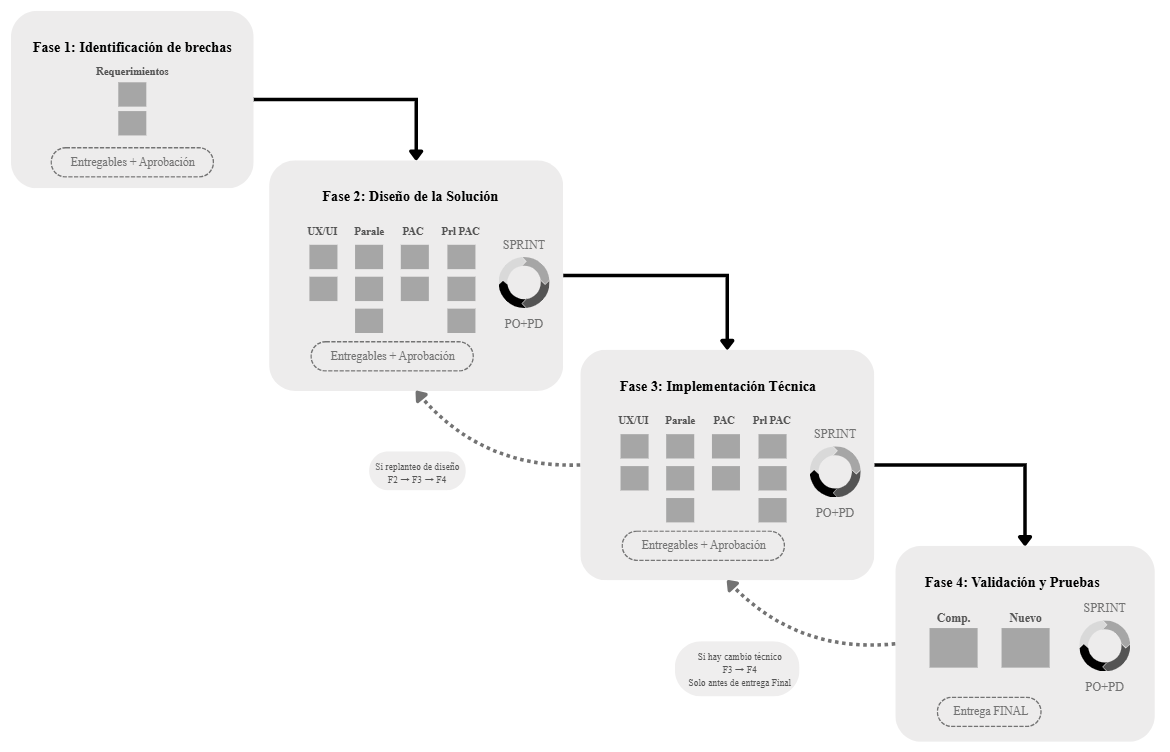
\includegraphics[width=\textwidth]{Ciclo de Vida GammaLab 2.0.png}
    \caption{Ciclo de vida metodológico adoptado para el desarrollo de GammaLab 2.0 bajo enfoque Water-Scrum-Fall.}
    \label{fig:ciclo_gammalab}
\end{figure}



\subsection{Proceso de Selección del Modelo de Ciclo de Vida}

El desarrollo de un sistema de software requiere, antes de cualquier decisión técnica, definir cómo se organizará el trabajo a lo largo del tiempo. Esta organización se formaliza a través de un modelo de ciclo de vida del software, que Pressman \& Maxim definen como una representación abstracta de la secuencia de actividades que guían al equipo desde la recolección de requisitos hasta la entrega y el mantenimiento del sistema \cite{pressman2015}.

En términos generales, los modelos de ciclo de vida se agrupan en dos grandes categorías: los modelos dirigidos por plan (plan-driven), donde todas las fases se planifican en detalle desde el inicio y el progreso se mide contra ese plan; y los modelos ágiles, donde la planificación es incremental y el proceso se adapta continuamente a los cambios del entorno y de los requisitos \cite{sommerville2016}. Entre estos dos extremos existe un espectro de variantes que difieren en aspectos como la secuencialidad de sus fases, el nivel de documentación exigido, la frecuencia de entrega de resultados y el grado de participación del cliente durante el desarrollo. A continuación se presenta una revisión de los modelos de mayor relevancia en la literatura, con el propósito de fundamentar la elección metodológica para el desarrollo de GammaLab 2.0.:

\begin{enumerate}
    \item \textbf{Modelo en cascada.} Propone una estrategia de organización estrictamente secuencial, en donde se propone el siguiente orden para los proyectos: requisitos, diseño, implementación, pruebas y mantenimiento. Se caracteriza porque en cada fase debe completarse y producir su documentación formal antes de iniciar la siguiente. Los recursos se asignan fase por fase, lo que típicamente implica equipos especializados por etapa con poca interacción cruzada. Es apropiado para proyectos grandes, con requisitos bien definidos desde el inicio, equipos distribuidos geográficamente y donde la documentación formal es un requisito contractual \cite{pressman2015}.
    \item \textbf{Modelo en V.} Se presenta como una extensión directa del modelo en cascada \cite{pressman2015}. Su diferencia central es que a cada fase de desarrollo le corresponde simétricamente una fase de verificación o prueba: los requisitos se asocian a pruebas de aceptación, el diseño del sistema a pruebas de integración, y el diseño detallado a pruebas unitarias. Los entregables y la documentación se generan en ambos lados de la V, lo que hace que el plan de pruebas se diseñe en paralelo al desarrollo desde las fases más tempranas. Al igual que la cascada, es un modelo rígido y secuencial, con equipos especializados por fase \cite{academia2012}.
    \item \textbf{Modelo incremental.} Combina elementos del modelo en cascada aplicados de forma iterativa y escalonada \cite{pressman2015}. El sistema se divide en incrementos funcionales que se desarrollan y entregan en secuencia; el primer incremento cubre la funcionalidad más crítica y cada entrega posterior añade capacidades adicionales. A diferencia de la cascada, los recursos se distribuyen de forma continua a lo largo del proyecto y los equipos son multifuncionales, trabajando especificación, diseño e implementación para cada incremento. La comunicación con el cliente es más frecuente al haber entregas periódicas \cite{sommerville2016}.
    \item \textbf{Modelo en espiral.} Se diferencia de los anteriores por centrar el proceso en la gestión del riesgo \cite{pressman2015}. El proyecto avanza en iteraciones cíclicas, cada vuelta de la espiral pasa por planificación, análisis de riesgos, desarrollo y evaluación y en cada ciclo el sistema se hace más completo. Los recursos se consumen de manera incremental por ciclo, lo que permite ajustar el alcance según los riesgos identificados. La documentación y los entregables se producen al final de cada iteración. Es apropiado para proyectos grandes, complejos, de larga duración y con alta incertidumbre técnica \cite{sommerville2016}.
     \item \textbf{Scrum.} Es un marco ágil que organiza el trabajo en ciclos cortos de duración fija llamados sprints, típicamente de dos a cuatro semanas, al final de los cuales se entrega un incremento funcional del producto \cite{schwaber2020}. Define tres roles claros: el Product Owner, que prioriza el trabajo; el Scrum Master, que facilita el proceso; y el equipo de desarrollo, que es pequeño, multifuncional y autogestionado. La documentación es ligera y los entregables son incrementos de software funcional evaluados en cada Sprint Review. La comunicación es intensiva y diaria dentro del equipo. Es recomendado para equipos pequeños  con requisitos cambiantes y acceso continuo al cliente \cite{pressman2015}.
\end{enumerate}

Con base en la revisión anterior, la siguiente tabla sintetiza las características más relevantes de cada modelo para efectos de la selección metodológica:


\begin{table}[h!]
\centering
\resizebox{\textwidth}{!}{
\begin{tabular}{|p{3cm}|p{2.2cm}|p{2.2cm}|p{2.2cm}|p{2.2cm}|p{2.2cm}|}
\hline
\textbf{Criterio} & \textbf{Cascada} & \textbf{Modelo V} & \textbf{Incremental} & \textbf{Espiral} & \textbf{Scrum} \\
\hline
\textbf{Documentación} & Extensa y formal por fase & Extensa, incluye plan de pruebas desde el inicio & Moderada por incremento & Moderada por iteración & Ligera, orientada a entregables funcionales \\
\hline
\textbf{Tamaño del proyecto} & Grande & Grande & Mediano & Grande y complejo & Pequeño a mediano \\
\hline
\textbf{Número de integrantes} & Equipos grandes y especializados & Equipos grandes y especializados & Equipos medianos multifuncionales & Equipos medianos con perfil en gestión de riesgos & Equipos pequeños (3--9 personas) \\
\hline
\textbf{Interacción con el cliente} & Baja, concentrada al inicio y al final & Baja, concentrada al inicio y al final & Media, en cada entrega incremental & Media, al cierre de cada iteración & Alta, continua durante los sprints \\
\hline
\textbf{Flexibilidad ante cambios} & Muy baja & Muy baja & Media & Alta por gestión de riesgos & Muy alta \\
\hline
\textbf{Testeo} & Al final del desarrollo & Planificado desde el inicio, paralelo al diseño & Al final de cada incremento & Al final de cada iteración & Continuo dentro de cada sprint \\
\hline
\textbf{Entrega de valor} & Única, al final del proyecto & Única, al final del proyecto & Parcial y progresiva & Parcial por iteración & Parcial al cierre de cada sprint \\
\hline
\end{tabular}
}
\caption{Comparación de modelos de ciclo de vida}
\label{tab:comparacion_modelos}
\end{table}

Al contrastar estas características con el contexto de GammaLab 2.0, se observa que ningún modelo satisface por sí solo las necesidades del proyecto. Por una parte, existen dependencias técnicas claramente secuenciales derivadas de los objetivos específicos: no es posible implementar sin antes diseñar la arquitectura, ni diseñar sin haber identificado y priorizado previamente las brechas. Esto evidencia la necesidad de una estructura por fases y cierto nivel de planificación anticipada.

Sin embargo, el proyecto también presenta condiciones que demandan flexibilidad. El equipo está conformado por cuatro integrantes, los requisitos funcionales continúan definiéndose durante el desarrollo y la interacción con el cliente es frecuente, con retroalimentación constante de la directora del proyecto. Estas características resultan incompatibles con la rigidez documental y la baja capacidad de adaptación de modelos como cascada y modelo en V.

Por otra parte, metodologías puramente ágiles como Scrum se ajustan mejor al tamaño del equipo y a la dinámica iterativa del trabajo, pero no proporcionan por sí solas una estructura suficientemente robusta para gestionar las dependencias entre las grandes etapas del proyecto.

Sommerville (2016) señala que, en la práctica, los procesos de software reales rara vez adoptan un único modelo de manera pura, sino que combinan elementos de enfoques dirigidos por plan y enfoques ágiles de acuerdo con las características y restricciones particulares de cada proyecto.  Yahya \& Maidin (2022) documentan empíricamente esta tendencia, observando que numerosos proyectos recurren a modelos híbridos que combinan la estructura secuencial de metodologías tradicionales con la flexibilidad iterativa de Scrum, configurando lo que se conoce como \textit{Water-Scrum-Fall}. Este enfoque conserva una organización global por fases, permitiendo gestionar dependencias técnicas y mantener trazabilidad sobre el avance del proyecto, mientras incorpora dinámicas ágiles al interior de cada etapa mediante trabajo iterativo, entregables parciales y retroalimentación continua \cite{yahya2022}.

Por estas razones, y en coherencia con las necesidades previamente identificadas para GammaLab 2.0, se selecciona Water-Scrum-Fall como el ciclo de vida metodológico más adecuado para el desarrollo del proyecto.

\subsection{Lenguajes y Herramientas}

Dado que GammaLab 2.0 corresponde a una evolución directa de GammaLab 1.0, el desarrollo técnico del proyecto prioriza la continuidad tecnológica y la reutilización de la arquitectura existente. Esta decisión responde al propósito de preservar el trabajo previamente realizado, mantener compatibilidad con los módulos implementados y reducir costos asociados a una reestructuración completa del sistema.

En este sentido, la mayoría de los lenguajes y herramientas empleados en GammaLab 1.0 se conservan para esta nueva versión. No obstante, GammaLab 2.0 incorpora mejoras orientadas a solucionar limitaciones identificadas en la versión anterior, particularmente relacionadas con estabilidad técnica, experiencia de usuario y extensión de funcionalidades para análisis de señales EEG.

La Tabla \ref{tab:herramientas_gammalab} resume el conjunto de tecnologías utilizadas en el desarrollo del proyecto.

\begin{table}[h!]
\centering
\begin{tabular}{|p{5cm}|p{7cm}|}
\hline
\textbf{Categoría} & \textbf{Tecnologías empleadas} \\
\hline
Lenguaje de programación & Python \\
\hline
Desarrollo de interfaz gráfica & PySide6, Qt Designer \\
\hline
Entorno de desarrollo & Visual Studio Code \\
\hline
Control de versiones & Git, GitHub \\
\hline
Gestión del proyecto & GitHub Projects \\
\hline
Documentación técnica & LaTeX (Overleaf), Microsoft Word \\
\hline
Pruebas & Pytest \\
\hline
Diseño de interfaz y diagramas & Figma, Draw.io, Canva \\
\hline
Comunicación y colaboración & Microsoft Teams, WhatsApp \\
\hline
Almacenamiento y respaldo & OneDrive, máquina virtual compartida \\
\hline
\end{tabular}
\caption{Lenguajes y herramientas empleadas en GammaLab 2.0}
\label{tab:herramientas_gammalab}
\end{table}

\textbf{Python} se mantiene como lenguaje principal del proyecto, dado que GammaLab fue originalmente desarrollado en este entorno y cuenta con compatibilidad directa con bibliotecas científicas ampliamente utilizadas en procesamiento de señales, como NumPy, SciPy, MNE-Python y PyEEG. Esto permite conservar la base existente e incorporar nuevas funcionalidades de análisis EEG sin modificar el ecosistema tecnológico principal.

Para la interfaz gráfica se conserva el uso de \textbf{PySide6} y \textbf{Qt Designer}, herramientas que permiten mantener coherencia con la arquitectura visual existente y facilitan la separación entre diseño de interfaz y lógica funcional.

En términos de desarrollo colaborativo, el proyecto utiliza \textbf{Git} y \textbf{GitHub} para control de versiones, gestión de ramas y revisión de cambios, complementados con \textbf{GitHub Projects} como herramienta de seguimiento de tareas acorde con la dinámica iterativa definida en la metodología del proyecto.

La documentación técnica y académica se desarrolla principalmente en \textbf{LaTeX mediante Overleaf}, favoreciendo trazabilidad, edición colaborativa y consistencia de formato. Adicionalmente, se emplea Microsoft Word para documentación preliminar y trabajo colaborativo informal.

Para diseño y modelado visual se utilizan \textbf{Figma} en prototipado de interfaces, \textbf{Draw.io} para diagramas técnicos y \textbf{Canva} para material gráfico de apoyo.

Finalmente, el aseguramiento de calidad incorpora pruebas mediante \textbf{Pytest}, mientras que la coordinación del equipo se apoya en \textbf{Microsoft Teams} y \textbf{WhatsApp}. Como mecanismo de respaldo y pruebas compartidas, el proyecto cuenta adicionalmente con almacenamiento en \textbf{OneDrive} y una máquina virtual compartida.

\subsection{Organización del proyecto y Comunicación}

La organización de GammaLab 2.0 responde a la naturaleza colaborativa e iterativa del proyecto, integrando una estructura ligera de coordinación alineada con el enfoque metodológico Water-Scrum-Fall adoptado.

A nivel organizacional, el cliente del proyecto corresponde al Laboratorio de Electrofisiología de la Universidad Nacional de Colombia, entidad beneficiaria del desarrollo y principal fuente de requerimientos funcionales y criterios de validación del sistema.

La directora del proyecto actua como puente de comunicación entre el equipo de desarrollo y el cliente. Sus responsabilidades incluyen facilitar la coordinación de reuniones con el laboratorio, orientar la toma de decisiones relacionadas con alcance, complejidad técnica y priorización funcional, así como ejercer supervisión técnica y académica sobre el desarrollo del proyecto. 

El equipo de desarrollo está conformado por cuatro integrantes, todos con participación activa en las distintas fases del proyecto. La distribución del trabajo se realiza de manera colaborativa y equitativa, asignando responsabilidades de acuerdo con los frentes funcionales definidos y promoviendo revisión cruzada entre integrantes para asegurar consistencia técnica e integración del sistema.

Adicionalmente, uno de los integrantes asume funciones equivalentes al rol de \textit{Scrum Master}, en calidad de líder del equipo. Este rol se enfoca en la coordinación general del trabajo, seguimiento del cronograma, organización de reuniones y monitoreo del avance del proyecto, sin implicar una carga adicional de desarrollo respecto a los demás integrantes. La ejecución técnica y cumplimiento de objetivos se mantiene distribuida de manera equitativa entre todos los miembros.

La comunicación formal del proyecto se realiza mediante reuniones periódicas con la directora, orientadas al seguimiento metodológico, revisión de avances y resolución de decisiones técnicas o estratégicas. De forma complementaria, el equipo mantiene canales de comunicación interna para coordinación diaria, seguimiento de tareas y gestión ágil de bloqueos operativos.

Esta estructura organizacional permite mantener claridad en la toma de decisiones, supervisión continua y comunicación efectiva con el cliente, preservando al mismo tiempo una dinámica horizontal y colaborativa dentro del equipo de desarrollo.

La estructura organizacional del proyecto se presenta en la Figura \ref{fig:organigrama_gammalab}.

\begin{figure}[H]
    \centering
    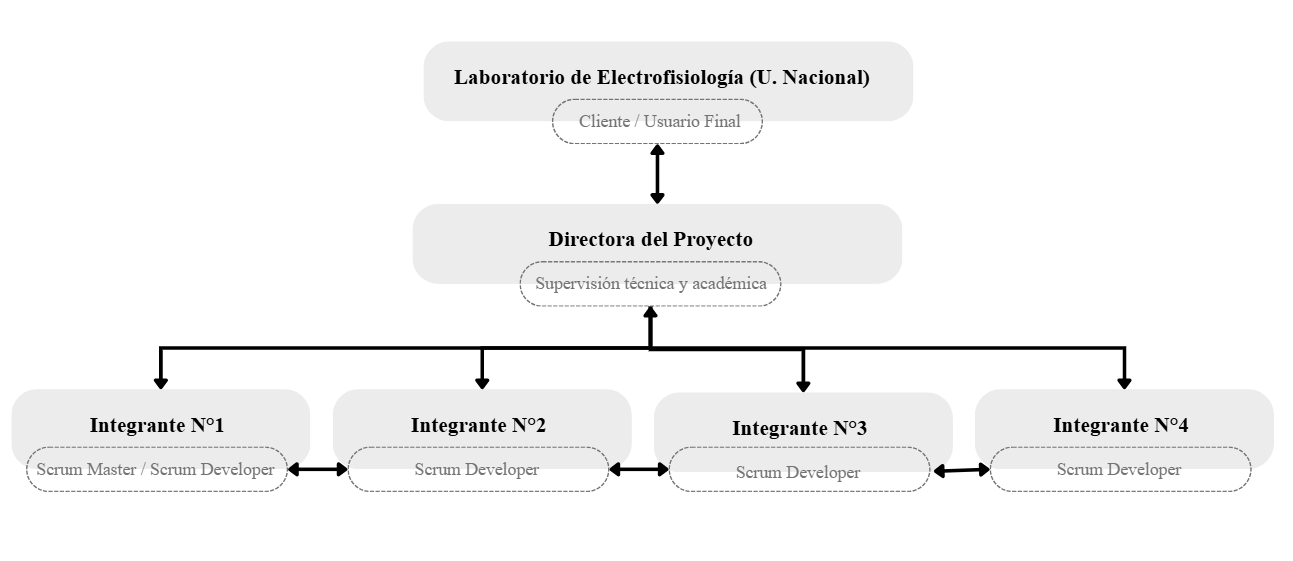
\includegraphics[width=\textwidth]{Organigrama GammaLab 2.0.png}
    \caption{Organigrama y Flujo de Comunicación del proyecto GammaLab 2.0}
    \label{fig:organigrama_gammalab}
\end{figure}



\subsection{Entregables del Proyecto}

Como resultado del desarrollo de GammaLab 2.0 bajo el enfoque metodológico definido, el proyecto contempla la generación de entregables técnicos, funcionales y documentales asociados a las distintas fases del ciclo de vida. Estos productos permiten evidenciar el cumplimiento progresivo de los objetivos específicos y consolidan tanto los resultados internos del desarrollo como los artefactos finales del proyecto.

\begin{itemize}[label={}]
    \item \textbf{Documento de análisis técnico y funcional de GammaLab 1.0.} 
    Consolida los hallazgos derivados de la exploración del código fuente, arquitectura y funcionalidades existentes, sirviendo como base para la identificación de oportunidades de mejora.

    \item \textbf{Product Backlog inicial priorizado.} 
    Contiene las brechas identificadas, organizadas y priorizadas de acuerdo con su impacto, viabilidad y alineación con los objetivos del proyecto.

    \item \textbf{Plan de pruebas de línea base y resultados iniciales.} 
    Define y documenta las pruebas aplicadas sobre GammaLab 1.0 para establecer métricas de referencia en rendimiento técnico y experiencia de usuario.

    \item \textbf{Artefactos de diseño y modelado.} 
    Incluye diagramas de casos de uso, diagramas de frecuencia, arquitectura de componentes y demás representaciones estructurales de GammaLab 2.0.

    \item \textbf{Prototipo de interfaz gráfica.} 
    Presenta la propuesta visual y de experiencia de usuario para GammaLab 2.0 antes de su implementación definitiva.

    \item \textbf{Documento de arquitectura de GammaLab 2.0.} 
    Formaliza las decisiones estructurales del sistema, incluyendo distribución de componentes y justificación técnica de diseño.

    \item \textbf{Especificaciones técnicas del nuevo módulo de análisis.} 
    Describe entradas, salidas, parámetros configurables y dependencias del nuevo módulo funcional incorporado en GammaLab 2.0.

    \item \textbf{Incrementos funcionales de software por sprint.} 
    Corresponden a avances parciales implementados y verificados al cierre de cada ciclo iterativo de desarrollo.

    \item \textbf{GammaLab 2.0 implementado.} 
    Versión final del sistema con integración de mejoras funcionales, optimizaciones técnicas y nuevos módulos de análisis.

    \item \textbf{Repositorio final organizado.} 
    Código fuente estructurado, versionado y documentado para facilitar mantenimiento, trazabilidad y futuras extensiones del proyecto.

    \item \textbf{Informes de validación y pruebas.} 
    Documentan resultados de pruebas técnicas, análisis comparativo entre GammaLab 1.0 y 2.0, y validación funcional de nuevas capacidades.

    \item \textbf{Manual de uso de GammaLab 2.0.} 
    Guía orientada al usuario final que describe instalación, navegación y uso de funcionalidades principales del sistema.

    \item \textbf{Documento final de memoria del proyecto.} 
    Consolida el proceso completo de desarrollo, incluyendo contexto, metodología, diseño, implementación, pruebas, resultados y conclusiones.

    \item \textbf{Entrega final al cliente.} 
    Compilación organizada de software, documentación y materiales complementarios entregados al Laboratorio de Señales.
\end{itemize}

\subsection{Estructura colaborativa y enfoque de trabajo}

\begin{table}[H]
\label{tab:roles_equipo}
\renewcommand{\arraystretch}{1.3}

\begin{tabular}{|p{3.5cm}|p{3.5cm}|p{4.5cm}|}
\hline
\textbf{Participante} & \textbf{Rol} & \textbf{Descripción del rol} \\ \hline

Laboratorio de Electrofisiología (U. Nacional) & Cliente / Entidad beneficiaria & Define necesidades funcionales, valida resultados y recibe la entrega final del proyecto. \\ \hline

Cécile Gauthier Umaña & Directora del proyecto & Puente de comunicación con el cliente, orienta decisiones estratégicas y supervisa el desarrollo técnico y académico. \\ \hline

Juan Felipe Romero & Scrum Master & Asume funciones de liderazgo y coordinación general del equipo, manteniendo participación activa en el desarrollo técnico del proyecto. \\ \hline

Juan Felipe Romero, Laura Juliana Garzón, Sebastian Almanza y Xiomara Herrera & Scrum Developers & Participan en actividades de diseño, implementación, integración, pruebas y documentación del sistema. \\ \hline

\end{tabular}
\centering
\caption{Distribución de roles del proyecto}
\end{table}

El desarrollo de GammaLab 2.0 se ejecuta bajo una dinámica de trabajo colaborativa, en la cual los cuatro integrantes participan activamente en las distintas fases del proyecto y comparten responsabilidad sobre el cumplimiento de los objetivos técnicos definidos. Aunque cada integrante asume liderazgo temporal sobre componentes específicos, el trabajo no se encuentra segmentado de manera rígida, sino que se favorece una distribución flexible de tareas según las necesidades de cada fase, el avance del proyecto y la complejidad técnica de los módulos involucrados. Esta estructura permite aprovechar las fortalezas individuales del equipo sin comprometer una visión integral del sistema.

Dentro de esta dinámica, el líder del equipo asume adicionalmente funciones de coordinación equivalentes al rol de \textit{Scrum Master}. Paralelamente, se promueve la revisión cruzada, validación conjunta de decisiones técnicas y apoyo colaborativo en procesos de integración, pruebas y resolución de bloqueos.

Este esquema de trabajo responde directamente al enfoque híbrido Water-Scrum-Fall adoptado, permitiendo mantener una estructura organizada por fases mientras se incorporan ciclos iterativos de trabajo y retroalimentación continua. Dicha retroalimentación puede provenir tanto del cliente, como principal fuente de validación funcional y requerimientos, como de la directora del proyecto, quien complementa este proceso mediante supervisión técnica y académica.

\section{Administración del Proyecto}

En esta sección se documentan los mecanismos de administración del proyecto GAMMA LAB 2.0, incluyendo estimación de actividades, inicio del proyecto, planes de trabajo, descomposición de actividades (WBS), calendarización, asignación de recursos y gestión de métricas.

\subsection{Métodos y Herramientas de Estimación}

Para la estimación de actividades del proyecto GAMMA LAB 2.0, se adopta un enfoque de estimación \textit{Bottom-Up}, el cual parte de la identificación de tareas específicas y granulares, estima el esfuerzo requerido para cada una de ellas, y posteriormente agrega estas estimaciones para obtener el tiempo total del proyecto. Esta metodología es particularmente adecuada para proyectos en evolución donde se cuenta con experiencia de una versión anterior y donde las dependencias técnicas son claras.

El proceso inició con la definición de las cuatro fases del proyecto, correlacionadas directamente a los cuatro objetivos específicos:

\begin{itemize}
    \item \textbf{Fase 1: Identificación de brechas de mejora en GammaLab 1.0} -- 3 semanas
    \item \textbf{Fase 2: Diseño del planteamiento estructural de la solución} -- 4 semanas
    \item \textbf{Fase 3: Implementación técnica} -- 7 semanas
    \item \textbf{Fase 4: Validación y pruebas con el usuario} -- 2 semanas
\end{itemize}

A partir de esta estructura, el equipo identificó las actividades concretas dentro de cada fase, desagregó estas actividades en tareas específicas y estimó el esfuerzo en horas-persona requerido para cada tarea. Esta información se consolidó en una tabla de estimación detallada que refleja la carga de trabajo esperada por fase.

\subsubsection{Supuestos de Estimación}

La estimación se fundamenta en los siguientes supuestos:

\begin{itemize}
    \item El equipo de desarrollo está compuesto por cuatro desarrolladores dedicados al 100\% del proyecto.
    \item Cada desarrollador dispone de un mínimo de 6 horas semanales de disponibilidad efectiva para trabajo de desarrollo, análisis, diseño, codificación y pruebas.
    \item La jornada semanal de dedicación será distribuida de manera flexible entre las actividades, con énfasis en mantener sincronización a través de canales de comunicación asíncrona (GitHub, comunicación escrita).
    \item Se reutilizará conocimiento y código de GAMMA LAB 1.0, reduciendo el tiempo de aprendizaje inicial.
    \item La directora del proyecto está disponible para sesiones de revisión semanal y proporciona retroalimentación en plazos acordados.
    \item El cliente (Laboratorio de Electrofisiología) participa activamente en validaciones de línea base (Fase 1) y en pruebas finales (Fase 4).
    \item No existen restricciones significativas de recursos técnicos o de infraestructura que impidan la ejecución del proyecto.
    \item Las metodologías de desarrollo (Water-Scrum-Fall) y las herramientas (Git, GitHub Projects, Python, PySide6) permanecen estables durante la ejecución.
\end{itemize}

\subsubsection{Estimación de Tiempo por Fases del Proyecto}

La siguiente tabla resume la estimación de duración por fases, con base en el análisis Bottom-Up de actividades y tareas:

\begin{table}[H]
\centering
\small
\begin{tabular}{|p{2cm}|p{3cm}|p{2cm}|p{2cm}|p{2cm}|}
\hline
\textbf{Fase} & \textbf{Descripción} & \textbf{Duración} & \textbf{Inicio} & \textbf{Cierre} \\
\hline
1 & Identificación de brechas & 3 sem & 27 jul & 16 ago \\
\hline
2 & Diseño de solución & 4 sem & 19 ago & 13 sep \\
\hline
3 & Implementación técnica & 7 sem & 16 sep & 27 oct \\
\hline
4 & Validación y pruebas & 2 sem & 28 oct & 20 nov \\
\hline
\multicolumn{2}{|l|}{\textbf{Total estimado}} & \textbf{16 sem} & \textbf{27 jul} & \textbf{20 nov} \\
\hline
\end{tabular}
\caption{Resumen de calendarización del proyecto GAMMA LAB 2.0}
\label{tab:calendario}
\end{table}

\subsubsection{Distribución de Esfuerzo por Fase}

Basado en el análisis Bottom-Up de tareas, la siguiente tabla detalla el esfuerzo estimado (en horas-persona) para cada fase:

\begin{table}[H]
\centering
\small
\begin{tabular}{|p{3.5cm}|p{2.5cm}|p{3cm}|}
\hline
\textbf{Fase} & \textbf{Duración (sem)} & \textbf{Esfuerzo Total (h-persona)} \\
\hline
Fase 1: Identificación de brechas & 3 & 72 h \\
\hline
Fase 2: Diseño de solución & 4 & 96 h \\
\hline
Fase 3: Implementación técnica & 7 & 168 h \\
\hline
Fase 4: Validación y pruebas & 2 & 48 h \\
\hline
\textbf{Total} & \textbf{16} & \textbf{384 h} \\
\hline
\end{tabular}
\caption{Estimación de esfuerzo por fases del proyecto (Bottom-Up)}
\label{tab:esfuerzo}
\end{table}

\textit{Nota: El esfuerzo total de 384 horas se distribuye entre 4 desarrolladores, resultando en 96 horas por persona en las 16 semanas, equivalentes a 6 horas semanales promedio por desarrollador.}

\subsection{Inicio del Proyecto}

\subsubsection{Entrenamiento del Personal}

El equipo de GAMMA LAB 2.0 está compuesto por cuatro desarrolladores nuevos, por lo que es fundamental un plan estructurado de transferencia de conocimiento y entrenamiento que les permita:

\begin{itemize}
    \item Comprender la arquitectura y funcionamiento de GAMMA LAB 1.0
    \item Familiarizarse con las tecnologías base (Python, PySide6, MNE-Python, etc.)
    \item Alinearse con los estándares de código y de documentación del proyecto
    \item Entender el dominio técnico (procesamiento de señales EEG, análisis en dominios de tiempo, frecuencia y tiempo-frecuencia)
\end{itemize}

El plan de entrenamiento se ejecutará durante la Fase 1 (primeras 3 semanas) de manera paralela a las actividades de análisis de brechas. Las actividades incluyen:

\begin{enumerate}
    \item \textbf{Sesiones de transferencia con equipo de GAMMA LAB 1.0:} Reuniones semiestructuradas donde el equipo original explica decisiones de diseño, limitaciones técnicas y funcionalidades planificadas pero no implementadas.
    
    \item \textbf{Exploración técnica autónoma:} Cada desarrollador realiza una revisión independiente del código fuente, arquitectura y documentación de GAMMA LAB 1.0, generando notas y preguntas que se resuelven en sesiones grupales.
    
    \item \textbf{Capacitación en dominio (EEG y procesamiento de señales):} Sesiones cortas sobre conceptos clave de electroencefalografía, análisis en dominios de tiempo, frecuencia y tiempo-frecuencia, así como sobre las nuevas técnicas que se implementarán (amplitude coupling, paralelización).
    
    \item \textbf{Alineación en estándares y herramientas:} Revisión de estándares de código (PEP8), políticas de control de versiones (Git, Pull Requests), estructura de repositorio y convenciones de documentación.
    
    \item \textbf{Sesiones de lluvia de ideas colaborativa:} El equipo completo (desarrolladores, directora, y ocasionalmente el cliente) participa en sesiones para alinear la visión del proyecto y clarificar alcances y expectativas.
\end{enumerate}

\subsubsection{Infraestructura}

Para el desarrollo de GAMMA LAB 2.0, se dispone de la siguiente infraestructura técnica y de colaboración:

\textbf{Infraestructura física:}
\begin{itemize}
    \item Cada desarrollador cuenta con su propio equipo de desarrollo (laptop o computadora de escritorio) con capacidad suficiente para programación, ejecución de código Python y pruebas locales.
    \item Se solicita acceso a una máquina virtual compartida que actúe como entorno de integración centralizado, permitiendo verificar compatibilidad multiplataforma y ejecutar pruebas de integración antes de la entrega final.
\end{itemize}

\textbf{Infraestructura lógica y de colaboración:}
\begin{itemize}
    \item \textbf{Control de versiones:} Git con repositorio centralizado en GitHub. La estructura del repositorio se basa en ramas por frente de trabajo (UI/UX, paralelización núcleo, amplitude coupling, paralelización módulo nuevo), con política de Pull Requests obligatoria para integración.
    
    \item \textbf{Entorno de desarrollo:} Visual Studio Code, PyCharm o editor de preferencia de cada desarrollador, con extensiones para linting (PEP8), debugging y testing.
    
    \item \textbf{Gestión del proyecto:} GitHub Projects en formato Kanban, con columnas: ``To Do'', ``In Progress'', ``In Review'', ``Done''. Sincronización asíncrona diaria a través de comentarios en tarjetas de tareas.
    
    \item \textbf{Comunicación:} Microsoft Teams para reuniones semanales formales con la directora; WhatsApp para coordinación ágil y resolución rápida de dudas.
    
    \item \textbf{Documentación técnica:} Overleaf para memoria del proyecto en LaTeX; Microsoft Word como herramienta auxiliar para redacción preliminar y colaboración paralela.
    
    \item \textbf{Prototipado y diseño:} Figma para diseño visual de la interfaz de usuario, con acceso compartido para revisión y validación iterativa.
    
    \item \textbf{Pruebas automatizadas:} Pytest como framework para pruebas unitarias, con configuración para ejecución local en cada desarrollo y en la máquina virtual compartida.
    
    \item \textbf{Respaldo y almacenamiento:} OneDrive para documentos y respaldo incremental; GitHub como respaldo de código fuente. Se ejecutará una política semanal de respaldo completo de código, documentación y artefactos del proyecto.
\end{itemize}





\subsection{Asignación de Recursos}

\subsubsection{Equipo de Desarrollo}

El equipo de GAMMA LAB 2.0 está conformado por cuatro estudiantes de Ingeniería de Sistemas de la Pontificia Universidad Javeriana, todos dedicados al 100\% del proyecto durante las 16 semanas de ejecución.

\begin{table}[H]
\centering
\small
\begin{tabular}{|p{2.8cm}|p{2.5cm}|p{1.5cm}|p{2.5cm}|}
\hline
\textbf{Nombre} & \textbf{Rol} & \textbf{Ded.} & \textbf{Responsabilidad} \\
\hline
Juan Felipe Romero Ortiz & Desarrollador + Scrum Master & 100\% & Frente 1 (UX/UI) \\
\hline
Laura Juliana Garzón Arias & Desarrollador & 100\% & Frente 2 (Paralelización) \\
\hline
Xiomara Herrera Suárez & Desarrollador & 100\% & Frente 3 (Amplitude Coupling) \\
\hline
Sebastian Almanza Galvis & Desarrollador & 100\% & Frente 4 (Paralelización módulo) \\
\hline
\end{tabular}
\caption{Equipo de desarrollo de GAMMA LAB 2.0}
\label{tab:equipo}
\end{table}

\textbf{Notas sobre asignación de roles:}

\begin{itemize}
    \item El rol de Scrum Master es asumido por Juan Felipe Romero Ortiz sin que esto implique jerarquía en la toma de decisiones. Sus responsabilidades incluyen agendar reuniones, dar seguimiento al progreso visible en GitHub Projects, mantener el enfoque del equipo y facilitar la comunicación con la directora.
    
    \item La distribución de tareas en cada sprint se define colectivamente mediante consenso del equipo, considerando las especialidades, la carga actual y las dependencias entre frentes de trabajo.
    
    \item Cada desarrollador es responsable de código de calidad (según PEP8), de incluir pruebas unitarias para sus cambios, y de participar activamente en revisión de código de sus compañeros.
    
    \item La asignación a frentes de trabajo no es exclusiva; los desarrolladores colaborarán entre frentes según las necesidades de cada sprint.
\end{itemize}

\subsubsection{Disponibilidad Horaria por Desarrollador}

Cada desarrollador dispone de un mínimo de 6 horas semanales de dedicación efectiva al proyecto. Esta disponibilidad se distribuye de la siguiente manera:

\begin{table}[H]
\centering
\small
\begin{tabular}{|p{3cm}|p{1.8cm}|p{2cm}|p{2.5cm}|}
\hline
\textbf{Desarrollador} & \textbf{Horas/sem} & \textbf{Total (16 sem)} & \textbf{Promedio por fase} \\
\hline
Juan Felipe Romero & 6 & 96 h & 24-28 h \\
\hline
Laura Juliana Garzón & 6 & 96 h & 24-28 h \\
\hline
Xiomara Herrera & 6 & 96 h & 24-28 h \\
\hline
Sebastian Almanza & 6 & 96 h & 24-28 h \\
\hline
\textbf{Total equipo} & \textbf{24} & \textbf{384 h} & \textbf{96-112 h} \\
\hline
\end{tabular}
\caption{Distribución de disponibilidad horaria por desarrollador}
\label{tab:disponibilidad}
\end{table}

\textbf{Gestión de disponibilidad:}

\begin{itemize}
    \item La dedicación es flexible en términos de distribución semanal, permitiendo que algunos desarrolladores trabajen más horas en semanas con dependencias críticas y menos en semanas de menor carga.
    
    \item Se espera que los desarrolladores comuniquen anticipadamente cualquier conflicto o reducción temporal en disponibilidad, para permitir que el equipo se reorganice.
    
    \item Las reuniones formales (Sprint Planning, Sprint Review, Sprint Retrospective, reuniones con directora) son obligatorias y están fuera de las 6 horas semanales de desarrollo estimadas. Se espera que no superen 2 horas semanales en total.
    
    \item La comunicación asíncrona a través de GitHub Issues, Pull Request comments y WhatsApp reduce la necesidad de reuniones en tiempo real, permitiendo máxima flexibilidad horaria.
\end{itemize}

\subsubsection{Directora del Proyecto}

\begin{table}[H]
\centering
\small
\begin{tabular}{|p{4cm}|p{3cm}|p{2cm}|}
\hline
\textbf{Nombre} & \textbf{Rol} & \textbf{Dedicación} \\
\hline
Cecile Eugenie Gloria Gauthier Umaña & Directora + Product Owner & 10\% \\
\hline
\end{tabular}
\caption{Directora del proyecto}
\label{tab:directora}
\end{table}

\textbf{Responsabilidades de la directora:}

\begin{itemize}
    \item Actúa como Product Owner, representando los intereses del cliente (Laboratorio de Electrofisiología) y priorizando el Product Backlog.
    
    \item Participa en Sprint Planning y Sprint Review semanales para alineación y validación.
    
    \item Proporciona retroalimentación sobre artefactos de diseño, código y documentación en plazos acordados (máximo 48 horas).
    
    \item Facilita comunicación entre el equipo de desarrollo y el cliente, recogiendo feedback y necesidades emergentes.
    
    \item Asegura el cumplimiento de estándares de calidad y de alineación con los objetivos planteados.
\end{itemize}

\subsubsection{Cliente}

\begin{table}[H]
\centering
\small
\begin{tabular}{|p{4cm}|p{3cm}|p{2.5cm}|}
\hline
\textbf{Entidad} & \textbf{Rol} & \textbf{Participación} \\
\hline
Laboratorio de Electrofisiología - Universidad Nacional de Colombia & Usuario final + Validador & Fases 1, 2, 4 \\
\hline
\end{tabular}
\caption{Cliente del proyecto}
\label{tab:cliente}
\end{table}

\textbf{Puntos de contacto con el cliente:}

\begin{itemize}
    \item \textbf{Fase 1:} Sesión formal de levantamiento de requerimientos, ejecución de pruebas de línea base sobre GAMMA LAB 1.0.
    
    \item \textbf{Fase 2:} Validación de prototipo de interfaz de usuario y especificaciones técnicas del nuevo módulo.
    
    \item \textbf{Fase 4:} Participación en pruebas funcionales, validación de amplitude coupling, pruebas de usabilidad y firma de aceptación final.
\end{itemize}

\subsection{Gestión de Cambios y Control de Alcance}

\subsubsection{Solicitudes de Cambio}

Durante el desarrollo, pueden surgir solicitudes de cambio de requerimientos, modificaciones de diseño o ajustes de alcance. Estas se manejan mediante el siguiente protocolo:

\begin{enumerate}
    \item \textbf{Identificación:} El cambio es identificado por cualquier miembro del equipo o del cliente.
    
    \item \textbf{Documentación:} Se crea una GitHub Issue con descripción clara del cambio, justificación e impacto estimado.
    
    \item \textbf{Evaluación:} El equipo y la directora evalúan el impacto en cronograma, recursos y alcance.
    
    \item \textbf{Priorización:} El cambio se añade al Product Backlog con prioridad asignada por consenso.
    
    \item \textbf{Integración:} El cambio se integra en el sprint siguiente si es de alta prioridad, o se pospone si afecta significativamente el cronograma.
\end{enumerate}

Cambios solicitados después de la mitad de Fase 3 (después del sprint 7) serán evaluados para versiones futuras, priorizando la entrega a tiempo de los objetivos planteados.

\subsection{Criterios de Éxito del Proyecto}

El proyecto GAMMA LAB 2.0 será considerado exitoso cuando se cumplan los siguientes criterios cuantificables:

\begin{enumerate}
    \item \textbf{Rendimiento mejorado:} GAMMA LAB 2.0 debe procesar señales EEG significativamente más rápido que GAMMA LAB 1.0. Se espera una mejora de al menos 20-30\% en tiempos de procesamiento derivada de la paralelización del sistema.
    
    \item \textbf{Nuevas funcionalidades correctas al 100\%:} El módulo de amplitude coupling debe operar sin errores críticos y producir resultados reproducibles y validables. Las pruebas unitarias deben pasar al 100\%.
    
    \item \textbf{Corrección de problemas de v1.0:} Los errores identificados en GAMMA LAB 1.0 que fueron priorizados en el Product Backlog (Fase 1) deben ser corregidos y validados por el cliente.
    
    \item \textbf{Validación de usuario:} El usuario final (Laboratorio de Electrofisiología) debe confirmar en la Fase 4 que:
    \begin{itemize}
        \item Las nuevas funcionalidades responden a sus necesidades.
        \item El sistema es intuitivo y fácil de usar.
        \item Los resultados del análisis son precisos y confiables.
        \item La documentación y manuales son claros.
    \end{itemize}
    
    \item \textbf{Cobertura de pruebas:} Mínimo 80\% cobertura de código en pruebas unitarias. Todo código nuevo debe incluir casos de prueba.
    
    \item \textbf{Documentación completa:} Memoria del proyecto con todas las secciones requeridas, manuales técnico y de usuario, comentarios en código y docstrings en funciones Python.
    
    \item \textbf{Entrega a tiempo:} El proyecto debe cerrar el 20 de noviembre de 2026 con todos los entregables completados según este PMP.
\end{enumerate}

\subsection{Monitoreo y Métricas de Avance}

\subsubsection{Métrica Clave: Velocidad del Equipo}

La \textit{velocidad} se define como el número de horas-persona completadas (según Definition of Done) por sprint. Esto permite:

\begin{itemize}
    \item Proyectar si el equipo completará el proyecto a tiempo.
    \item Identificar cuellos de botella u obstáculos.
    \item Ajustar la distribución de trabajo en sprints futuros.
\end{itemize}

\textbf{Seguimiento de velocidad:}

\begin{table}[H]
\centering
\small
\begin{tabular}{|p{3.5cm}|p{2.5cm}|p{2cm}|p{2cm}|}
\hline
\textbf{Métrica} & \textbf{Objetivo} & \textbf{Frecuencia} & \textbf{Responsable} \\
\hline
Velocidad por sprint & 24 h/semana & Semanal & Scrum Master \\
\hline
Burn-down chart & Progresión lineal & Semanal & Scrum Master \\
\hline
Definition of Done & 100\% cumplimiento & Por ítem & Equipo \\
\hline
Tasa de defectos & Minimizar & Por sprint & Testing \\
\hline
\end{tabular}
\caption{Métricas clave de monitoreo}
\label{tab:metricas}
\end{table}

\subsubsection{Reuniones de Sincronización}

\begin{itemize}
    \item \textbf{Sprint Planning:} Lunes de cada semana, 30 minutos. Selección de tareas del backlog y distribución entre desarrolladores.
    
    \item \textbf{Sincronización asíncrona:} Diariamente a través de comentarios en GitHub Issues. Cada desarrollador actualiza el estado de sus tareas.
    
    \item \textbf{Sprint Review:} Viernes de cada semana, 45 minutos. Presentación de incrementos completados a la directora. Retroalimentación.
    
    \item \textbf{Sprint Retrospective:} Viernes de cada semana (después de Review), 30 minutos. Análisis interno del equipo sobre qué funcionó bien, qué mejorar, y acciones correctivas para próximo sprint.
    
    \item \textbf{Sesiones técnicas:} Según necesidad (no planificadas regularmente). Para resolver decisiones arquitectónicas, resolver bloqueos o validaciones cruzadas entre frentes.
\end{itemize}

\section{Monitoreo y Control del Proyecto}

%--------------------------------------------------------------------
\subsection{Análisis y Administración de Riesgos}

\subsubsection{Proceso de gestión de riesgos}
Para el proceso de gestión de riesgos durante la realización de la tesis, el grupo seguirá los siguientes pasos:
\begin{itemize}
    \item \textbf{Identificación:} Detectar el o los eventos que afecten con el cronograma, la calidad o el alcance del proyecto.
    \item \textbf{Evaluación:} Clasificar el riesgo por su probabilidad (bajo, medio o alto) e impacto (ninguno, medio o alto).
    \item \textbf{Plan de respuesta:} Definir acciones de migración (para evitar que ocurra) o de contingencia (qué hacer si ocurre).
\end{itemize}

\subsubsection{Identificación de riesgos}
\begin{table}[!ht]
\begin{tabular}{ | m{3cm} | m{2.5cm} | m{2.5cm} | m{3cm} |}
\hline Riesgo & Probabilidad & Impacto & Mitigación \\ \hline
 Limitaciones de concurrencia en Python: El Global Interpreter Lock (GIL) podría impedir la mejora de desempeño esperada. & Alto & Alto & Investigar librerías de multiprocesamiento (multiprocessing) en lugar de hilos (threading) desde la Fase 2. \\ \hline
 Complejidad de integración: Dificultad para integrar el nuevo módulo de PAC con el núcleo "Microkernel" heredado de la v1.0. & Medio & Medio & Realizar una exploración técnica profunda en la Fase 1 y aplicar revisiones de código cruzadas.\\ \hline
 Baja disponibilidad horaria: El equipo solo dedica 6 horas semanales por persona, lo que deja poco margen para imprevistos. & Alto & Alto & Mantener conversaciones constantes por el grupo de WhatsApp y usar el "buffer" de los springs. \\ \hline
 Dependencia de stakeholders: Retrasos en la validación o consulta por parte del laboratorio. & Medio & Medio & Agendar sesiones de validación o consulta con 15 días de anticipo. \\ \hline
 Acceso a datos: No contar con señales EEG reales para las pruebas de validación. & Bajo & Alto & Se solicitarán varios datos de pruebas tanto al laboratorio como a la directora. \\ \hline
\end{tabular}
\caption{Tabla de riesgos}
\end{table}

\subsubsection{Matriz de respuesta}
En caso de que un integrante del grupo identifique un riesgo debera seguir los siguientes pasos:
\begin{itemize}
    \item \textbf{Notificar:} Tendrá que avisar lo antes posible al grupo por medio del grupo de WhatsApp o medio verbal.
    \item \textbf{Evaluación del impacto:} Se revisa si el camino crítico del diagrama de Gantt se ve afectado.
     \item \textbf{Ajuste de Backlog:} Si el riesgo afecta los tiempos de entrega, se reorganizará la entrega para asegurar cumplir los objetivos mínimos.
\end{itemize}


\subsection{Administración de Configuración y Documentación}
La administración de documentos y códigos se realizara mediante GitHub. El repositorio contendrá lo siguiente organizado en carpetas:
\begin{itemize}
    \item Documentación técnica del proyecto.
    \item Diagramas, manuales de uso y artefactos generados.
    \item Historial de versiones.
    \item Control de cambios.
\end{itemize}

\subsection{Métricas y Proceso de Medición}
La medición del avance y calidad del proyecto se realizara con las siguientes métricas:

\begin{table}[!ht]
\centering
\small
\begin{tabular}{|p{3.5cm}|p{5.5cm}|p{2.5cm}|p{2.5cm}|}
\hline
\textbf{Métrica} & \textbf{Descripción} & \textbf{Frecuencia} & \textbf{Herramienta} \\ \hline
IVE (Índice de Velocidad) & Relación entre las horas-persona ejecutadas frente a las 24 horas semanales planeadas por el equipo. & Semanal & GitHub Projects \\ \hline
Avance de Sprints & Porcentaje de ítems del Backlog completados (según el \textit{Definition of Done}) al cierre de cada ciclo. & Semanal & Burnup Chart (GitHub) \\ \hline
Cumplimiento de Hitos & Trazabilidad del avance de las 4 fases principales respecto a las fechas del cronograma. & Al cierre de fase & Hoja de control / Gantt \\ \hline
\end{tabular}
\caption{Métricas de progreso}
\label{tab:metricas_progreso}
\end{table}

\begin{table}[!ht]
\centering
\small
\begin{tabular}{|p{3.5cm}|p{5.5cm}|p{2.5cm}|p{2.5cm}|}
\hline
\textbf{Métrica} & \textbf{Descripción} & \textbf{Frecuencia} & \textbf{Herramienta} \\ \hline
Cobertura de Código & Porcentaje de código nuevo en Python que cuenta con pruebas unitarias asociadas . & Por incremento & Pytest \\ \hline
Mejora de Eficiencia ($E$) & Comparación porcentual del tiempo de procesamiento entre v1.0 y v2.0 ). & Fase 4 & Scripts de Benchmark \\ \hline
Trazabilidad de Requisitos & Porcentaje de funcionalidades del nuevo módulo de PAC y arquitectura validadas contra el diseño original. & Quincenal & Matriz de Trazabilidad \\ \hline
Validación del Cliente & Cantidad de observaciones críticas o sugerencias de mejora recibidas del Laboratorio de Electrofisiología. & Por prototipo & Formatos de revisión / Figma \\ \hline
\end{tabular}
\caption{Métricas de calidad}
\label{tab:metricas_calidad}
\end{table}

\subsection{Controles de Calidad}
Para evitar la acumulación de trabajo, se estableció un estándar de "Definition of Done" (DoD). Este conjunto de criterios establece que el producto de software debe pasar ciertos elementos antes de ser presentado en el spring. Un elemento se considera finalizado cuando cumple los siguientes requisitos:
\begin{itemize}
    \item El código ha sido sometido a una revisión cruzada (peer review) por un integrante diferente al que realizó la tarea, cumpliendo los estándares PEP8.
    
    \item La nueva funcionalidad se integra perfectamente en la rama principal del repositorio GitHub.
    \item Se actualiza la documentación del proyecto.
\end{itemize}

\begin{table}[!ht]
\centering
\small
\begin{tabular}{|p{3.5cm}|p{5cm}|p{3cm}|p{2.5cm}|}
\hline
\textbf{Actividad de Control} & \textbf{Descripción} & \textbf{Estándar / Herramienta} & \textbf{Responsable} \\ \hline
Revisión de Código (Peer Review) & Antes de integrar cualquier funcionalidad, otro integrante debe revisar la lógica y el estilo. & PEP8 / GitHub Pull Requests & Equipo de Desarrollo \\ \hline
Pruebas Unitarias Automatizadas & Verificación de que cada función nueva entregue resultados correctos y reproducibles. & Pytest / ISO/IEC 29119 & Scrum Developer \\ \hline
Análisis de Atributos de Calidad & Evaluación del rendimiento técnico (eficiencia) y la usabilidad de la nueva interfaz. & ISO/IEC 25010 & Scrum Master / Directora \\ \hline
Validación con el Cliente & Sesiones de prueba con investigadores del Laboratorio para confirmar utilidad y facilidad de uso. & Protocolo UAT / ISO 9241-11 & Product Owner / Cliente \\ \hline
\end{tabular}
\caption{Controles de Calidad de GammaLab 2.0}
\label{tab:controles_calidad}
\end{table}




\clearpage


\section{Monitoreo y Control del Proyecto}
En esta sección se describen los procesos y mecanismos para administrar
los requerimientos, monitorear el progreso, gestionar riesgos y realizar el cierre
formal del proyecto GAMMA LAB 2.0.

\subsection{Administración de Requerimientos}

\subsubsection*{Descripción del proceso}

La administración de requerimientos en GAMMA LAB 2.0 se concibe como un
proceso iterativo y controlado que permite gestionar los cambios de forma
ordenada y trazable a lo largo del ciclo de vida del proyecto bajo el enfoque
Water-Scrum-Fall. Este proceso involucra tanto al equipo de desarrollo con responsabilidades claras para la identificación,
documentación, revisión y validación de los requerimientos funcionales y no
funcionales del sistema.

La gestión de requerimientos comienza en la Fase~1, donde se identifican
brechas de mejora a través de exploración técnica de GammaLab~1.0,
entrevistas semiestructuradas con el equipo original y sesiones formales de
levantamiento de requerimientos con el cliente. Posteriormente, estos
requerimientos se modelan en casos de uso, se priorizan en el Product Backlog
y se documentan formalmente. Cada requerimiento se asocia a una matriz de
trazabilidad que permite vincularlo con componentes del diseño, código,
pruebas y entregables.

Durante el desarrollo iterativo (sprints), los requerimientos pueden ser refinados con base a una constante retroalimentación. El proceso de control incluye:

\begin{itemize}
    \item Un canal formal de solicitud de cambio.
    \item Evaluación del impacto técnico y temporal sobre el cronograma.
    \item Aprobación del cambio por consenso del equipo y la directora del proyecto.
    \item Actualización de todos los artefactos afectados: Product Backlog,
          documentos, matriz de trazabilidad, prototipos y código.
\end{itemize}

Los cambios solicitados después de la mitad de la Fase~3 (sprint~7) serán
evaluados para versiones futuras, priorizando la entrega a tiempo de los
objetivos planteados.

\subsubsection*{Artefactos por generar}

Durante la administración de requerimientos se generarán los siguientes
artefactos:

\begin{table}[!ht]
\centering
\small
\begin{tabular}{|p{4cm}|p{10cm}|}
\hline
\textbf{Artefacto} & \textbf{Descripción} \\ \hline

Product Backlog inicial & Lista priorizada de brechas y requerimientos identificados, acordados con el cliente al cierre de la Fase~1. \\ \hline

Casos de uso & Diagramas y descripciones narrativas que modelan las interacciones del usuario con el sistema para cada frente de trabajo. \\ \hline

Matriz de trazabilidad & Tabla que relaciona requerimientos con elementos de diseño, código y pruebas para garantizar cobertura completa. \\ \hline

Registro de solicitudes de cambio & documentación cada solicitud de cambio con su justificación, impacto estimado y estado de resolución. \\ \hline

Historial de versiones & Registro en GitHub que documenta los cambios aceptados en el repositorio y su justificación técnica. \\ \hline

\end{tabular}
\caption{Artefactos generados durante la administración de requerimientos}
\label{tab:artefactos_requerimientos}
\end{table}

\subsection{Monitoreo y Control de Progreso}

El seguimiento del progreso del proyecto se realizará mediante un sistema
combinado de control visual, medición de métricas clave y reportes
periódicos. El objetivo de este monitoreo es asegurar que el desarrollo se
mantenga alineado con los tiempos, entregables y objetivos definidos en la
planificación bajo el enfoque Water-Scrum-Fall.

Para ello, se implementarán tres estrategias complementarias:

\begin{itemize}
    \item \textbf{Diagrama de Gantt:} permite observar la duración y el
    solapamiento de actividades, así como su estado de avance en relación
    con la línea temporal del proyecto.

    \item \textbf{Burnup Chart en GitHub:} herramienta gráfica que compara
    el avance real frente al avance planificado en horas-persona, útil para
    identificar retrasos o desviaciones respecto a la velocidad objetivo del equipo.

    \item \textbf{Tablero Kanban en GitHub Projects:} muestra el estado del
    trabajo (\textit{To Do}, \textit{In Progress}, \textit{In Review},
    \textit{Done}), facilitando la identificación de bloqueos y la
    sincronización asíncrona diaria del equipo.
\end{itemize}

\begin{table}[H]
\centering
\small
\begin{tabular}{|p{4.5cm}|p{3cm}|p{2.5cm}|p{3.5cm}|}
\hline
\textbf{Actividad} & \textbf{Responsable} & \textbf{Frecuencia} & \textbf{Herramienta} \\ \hline

Actualización del tablero Kanban & Todo el equipo & Diaria & GitHub Projects \\ \hline

Verificación de velocidad del sprint &  Scrum Master & Semanal & GitHub Projects \\ \hline

Registro de desvíos y acciones correctivas & Scrum Master & Semanal & Hoja de seguimiento \\ \hline

Sprint Review con la directora & Equipo y Directora & Semanal (viernes) & Burnup Chart \\ \hline

Revisión del avance por fase & Directora del proyecto & Al cierre de fase & Gantt + Checklist \\ \hline

\end{tabular}
\caption{Actividades de monitoreo y responsables}
\label{tab:monitoreo_control}
\end{table}


\subsection{Cierre del Proyecto}

El cierre del proyecto contempla una serie de actividades orientadas a
garantizar la entrega formal, validación y documentación del producto
final. Las actividades clave serán:

\begin{itemize}
    \item \textbf{Sprint Review final:} presentación de los resultados
    comparativos entre GammaLab~1.0 y~2.0, y validación de las
    funcionalidades nuevas con la directora del proyecto.

    \item \textbf{Evaluación post-mortem del ciclo:} reflexión grupal sobre
    aprendizajes, errores y oportunidades de mejora para versiones futuras.

    \item \textbf{Revisión final de entregables:} verificación de
    completitud, actualización y correcta documentación de todos los
    artefactos del proyecto.

    \item \textbf{Prueba final del sistema:} ejecutada en condiciones reales
    de uso con investigadores del Laboratorio de Electrofisiología de la
    Universidad Nacional de Colombia.

    \item \textbf{Entrega formal del software:} incluye instalador, código
    fuente organizado, manual técnico y manual de usuario de GammaLab~2.0.

    \item \textbf{Firma de aceptación del cliente:} acta de conformidad
    posterior a la validación del sistema por parte del laboratorio.

    \item \textbf{Consolidación de documentación:} almacenamiento definitivo
    de todos los entregables en OneDrive y GitHub con tags de versión final.
\end{itemize}

\subsection{Entrega del Producto}

La entrega de GAMMALABalcliente se realizará durante la semana 17 del calendario
académico Javeriana 2026-30, correspondiente al cierre de la Fase~4 según el
calendario del proyecto. Se entregará el código fuente, los manuales
técnicos y las guías de usuario. El equipo de desarrollo será responsable
de realizar la instalación del sistema en los equipos del Laboratorio de
Electrofisiología que cuenten con sistema operativo compatible.

Una vez instalado, se ejecutará una prueba funcional con datos reales del
laboratorio. Se evaluará también la usabilidad del sistema mediante
sesiones guiadas y no guiadas con los investigadores, contrastando los
resultados frente a la línea base establecida en la Fase~1.





%--------------------------------------------------------------------
\begin{thebibliography}{00}

\bibitem{pressman2015}
R. S. Pressman and B. R. Maxim, \textit{Software Engineering: A Practitioner's Approach}, 8th ed. New York, NY, USA: McGraw-Hill Education, 2015.

\bibitem{schwaber2020}
K. Schwaber and J. Sutherland, \textit{The Scrum Guide: The Definitive Guide to Scrum: The Rules of the Game}. Scrum.org, 2020. [Online]. Available: https://scrumguides.org/docs/scrumguide/v2020/2020-Scrum-Guide-US.pdf

\bibitem{sommerville2016}
I. Sommerville, \textit{Software Engineering}, 10th ed. Harlow, England: Pearson Education, 2016.

\bibitem{yahya2022}
N. Yahya and S. S. Maidin, “The waterfall model with agile Scrum as the hybrid agile model for the software engineering team,” in \textit{2022 10th International Conference on Cyber and IT Service Management (CITSM)}, 2022, pp. 1--6, doi: 10.1109/CITSM56380.2022.9936036.

\bibitem{academia2012}
Academia.edu, “Comparative study of various process model in software development,” 2012. [Online]. Available: https://www.academia.edu/81531661

\end{thebibliography}
\end{document}
